%%%
%
% $Autor: Wings $
% $Datum: 2023-06-05 $
% $Dateiname: IMLSM9DS1 $
% $Version: 1 $
%
%%%

%% Structure
%\chapter{Sensor}
%
%
%\section{Specific Sensor}
%
%cite board
%
%\section{Specification}
%
%\begin{itemize}
%	\item cite data sheet
%	\item Circuit Diagram
%\end{itemize}
%
%\section{Library}
%
%\subsection{Description}
%
%\subsection{Installation}
%
%\subsection{Functions}
%
%\subsection{Example's Manual}
%
%\subsection{Inside the Example}
%
%\subsection{Example's Code}
%
%\subsection{Example's Files}
%
%
%
%\section{Calibration}
%
%cite method
%
%\section{Simple Code}
%
%
%\section{Simple Application}
%
%
%
%\section{Tests}
%
%\subsection{Simple Function Test}
%
%\subsection{Test all Functions}
%
%\section{Simple Application}
%
%
%\section{Further Readings}
%


\chapter{Sensor Inertial Measurement Unit}  \label{chap:InertialMeasurementUnit}

\section{General}
Inertial Measurement Units (IMU) are an essential component of many navigation and control systems. These devices integrate several sensors, including accelerometers and gyroscopes, to measure and track an object's movements in three-dimensional space. IMUs are widely used in a variety of applications, such as autonomous vehicle navigation, virtual reality, image stabilization, and even in wearable devices for tracking physical activity. Their ability to provide precise data on linear and angular acceleration makes them indispensable tools for systems requiring precise control and orientation, and ongoing technological advances have reduced their size, power consumption and cost, widening their scope of application in many fields. 
\cite{st_lsm9ds1:2025} \cite{analogdevices:2024} \cite{wahyudi:2011}


In addition to accelerometers and gyroscopes, IMUs may also include magnetometers, which measure the direction and strength of magnetic fields. These sensors can help provide additional information about the orientation and movement of an object in relation to Earth's magnetic field.\cite{Wang:2022}



\section{General Description }

The Inertial Measurement Unit is used to mesured acceleration or rotation, this is an electronic device which used three types of sensor magnetometer, accelerometer and gyroscope. These three sensors is used in LSM9DS1 and they give velocity, orientation and gravital force. 

The magnetometer measures the strength of magnetic fields, providing various types of information. For instance, when you pass a current through an electromagnet or generate a magnetic field in another way, the magnetometer can detect and quantify the strength of that field. \cite{st_microelectronics:2024}
\cite{STMicroelectronics_LSM9DS1:2024}\cite{sabatini:2011}





%%%%%%%%%%%%%%%%%%%%%%%%%%%%%%%%%%%%%%%%%%%%%%%%%%%%%%




\section{Errors}  \label{Chap: Errors}

\subsection{Introduction}

IMU (Inertial Measurement Unit) is a sensor that measures and reports the linear and rotational motion of an object. The error in IMU refers to any deviation or inaccuracy in the measurements reported by the sensor from the true or expected values.

\bigskip


\begin{enumerate}
	\item\textbf{Bias}: Bias is the constant offset in the readings of the IMU. It can be caused by a variety of factors, including manufacturing defects, aging of the sensors, or changes in temperature. These errors can lead to systematic errors that can persist over time and can be difficult to detect. To correct for the bias error, the IMU must be calibrated periodically. Calibration involves comparing the IMU's measurements with a known reference, and then estimating and subtracting the bias from the measurements to obtain more accurate results.\cite{sabatini:2011}
	
	\item \textbf{Drift}: Drift refers to the gradual change in bias over time. It can be caused by aging of the sensors, temperature changes, or electronic interference. Unlike the bias error, drift can vary over time, and it can be challenging to detect and correct. As a result, it is essential to calibrate the IMU regularly to correct for drift. More advanced techniques such as Kalman filtering can also be used to estimate and compensate for drift over time.\cite{Tedaldi:2014}
	
	\item \textbf{Noise:} Noise refers to the random variations in the sensor readings that can affect the accuracy of the measurement. This error is especially pronounced when the IMU is stationary. The noise can be caused by various factors such as electronic interference, vibrations, or environmental conditions. To reduce the noise error, various techniques such as filtering or averaging can be used. Filtering techniques can help remove random variations in the sensor readings and provide more accurate measurements. Averaging can also be used to reduce noise by averaging out random variations in the measurements over time.\cite{Faragher:2014}
\end{enumerate}

\subsection{Affected Parameters}
Bias, drift, and noise errors will affect all the accelerometers and gyroscopes parameters. Here's how they impact each parameter:

\subsubsection{Accelerometer:}

\begin{itemize}
	\item Ax, Ay, and Az: The accelerometer measures linear acceleration in three directions, X, Y, and Z. If the accelerometer experiences bias, there will be a constant offset in the acceleration measurement in all three directions, even when there is no actual acceleration. 
	\item Drift in an accelerometer can cause a slow, gradual change in the measured acceleration values over time. This means that even when the device is stationary, the accelerometer readings may drift away from the true acceleration values. For example, if the accelerometer is used to measure the tilt angle of a platform, drift can cause the tilt angle to slowly change even when the platform is not moving. Over time, this can result in significant errors in the measured tilt angle.
	\item Noise in an accelerometer can cause random fluctuations in the measured acceleration values. This means that even when the device is stationary, the accelerometer readings may vary randomly around the true acceleration values. For example, if the accelerometer is used to measure the vibration of a machine, noise can cause the measured vibration amplitude to fluctuate randomly around the true amplitude. This random fluctuation can make it difficult to accurately measure the machine's vibration characteristics.
\end{itemize}

\subsubsection{Gyroscope:}
\begin{itemize}
	\item $\Omega$x, $\Omega$y, and $\Omega$z: The gyroscope measures the rate of change of angular velocity in three directions, Roll, Pitch, and Yaw. Bias in the gyroscope can cause a constant offset in the measured angular velocity values, even when there is no actual rotation. \cite{Noureldin:2013}
	\item Drift in gyroscopes is caused by mechanical imperfections in the device, temperature changes, or other external factors that can lead to a gradual change in the measured angular velocity value over time, even when the device is not rotating. The drift error can accumulate over time and can significantly affect the accuracy of the gyroscope measurements. For example, a drone that uses a gyroscope for stabilization can experience drift error over time, causing it to drift off course and potentially crash.
	\item Noise in gyroscopes is caused by random fluctuations in the measured angular velocity values due to external disturbances such as vibrations or electromagnetic interference. The noise error can affect the precision of the gyroscope measurements and can lead to instability in the application. For example, in robotics, noise error can cause the robot to deviate from its intended path or make inaccurate movements.
\end{itemize}

To minimize these errors, calibration and filtering techniques can be used. Calibration can remove bias by using known reference values to adjust the sensor's measurements. Zero-g and zero-rate calibration techniques can be used to remove bias from accelerometers and gyroscopes, respectively. Filtering techniques can be used to remove noise and reduce drift. For example, a Kalman filter can be used to estimate the true acceleration or angular velocity values based on previous measurements and sensor models.\cite{Lin:2005}

%%%%%%%%%%%%%%%%%%%%%%%%%%%%%%%%%%%%%%%%%%%%%%%%%%%%%%%%%%%%%%%%


\section{Specific Sensor }
\subsection{LSM9DS1}

The LSM9DS1 sensor, engineered by STMicroelectronics, is a highly advanced 3-axis Inertial Measurement Unit (IMU) that incorporates a high-performance 3-axis digital accelerometer and 3-axis digital gyroscope. This meticulously crafted device is designed for precise motion tracking and finds extensive use in wearable devices and smartphones. With its capability to concurrently measure both linear and rotational motion, it stands as a benchmark in motion-sensing technology. \cite{STMicroelectronics_LSM9DS1:2024}

Developed to detect various types of motion, the LSM9DS1 sensor offers features such as stationary/motion detection, tilt sensing, pedometer functions, and timestamping. Additionally, it supports the integration of an external magnetometer, expanding its functionality further. The sensor provides hardware flexibility, allowing for different pin connections to external sensors. This flexibility enables the expansion of functionalities, such as adding a sensor hub or auxiliary SPI connections, to meet diverse application requirements.

\subsection{Always On Mode}

This feature implies that the LSM9DS1 can remain operational continuously, even when a device is in sleep mode, without excessively draining power. Such functionality proves invaluable for applications that require uninterrupted motion tracking, like fitness monitoring or navigation systems. \cite{st_microelectronics:2024}

\bigskip

The power consumption is an important factor when we have battery-powered device like smartphone. These devices need to be lightweight and portable, which requires minimizing battery weight and maximizing battery life.

\bigskip

The LSM9DS1 consumes only 0.55 mA when operating in combo high-performance mode. This low power consumption allows the sensor to deliver exceptional data quality while efficiently using battery power. In this mode, the sensor can simultaneously measure acceleration and angular rate, providing precise and reliable data even at high sampling rates.


\subsection{Tilt detection}

These features imply that tilt detection relies on the accelerometer to detect movement. When movement occurs, the tilt detection feature identifies it. Additionally, the tilt function operates with ultra-low power consumption. \cite{st_microelectronics:2024}

For example, if you have your smartphone in your front pant pocket, the tilt detection feature can determine whether you are moving from a standing to a sitting position or from sitting to standing.

\subsection{Significant Motion Detection}

This feature indicates that the Significant Motion Detection in the LSM9DS1 uses only the accelerometer to detect large movements.\cite{st_microelectronics:2024}


\subsection{Accelerometer}

The STMicroelectronics LSM9DS1 accelerometer is an advanced sensor crafted to measure linear acceleration along the x, y, and z axes. Its wide measurement range, spanning from ±2g to ±16g, ensures versatility across various applications. Boasting exceptional precision and reliability, it stands as a go-to choice for engineers and designers seeking accurate motion tracking solutions. \cite{STMicroelectronics_LSM9DS1:2024}
\bigskip 

Moreover, its low power consumption, typically ranging from 0.55 mA to 1.25 mA, makes it ideal for battery-powered devices. This feature ensures prolonged operation without draining excessive power, enhancing the efficiency and longevity of battery-powered systems.

\bigskip 

With an operating voltage range of 1.71 V to 3.6 V, the LSM9DS1 accelerometer easily adapts to different system configurations, offering flexibility in integration. Whether employed in wearable devices for motion tracking, drones for stabilization, or structural monitoring for vibration analysis, the LSM9DS1 accelerometer consistently delivers outstanding performance.

\bigskip 

Compact yet robust, the LSM9DS1 accelerometer is engineered to withstand demanding environments while providing precise and reliable measurements. Its reputation as a preferred choice among engineers and designers underscores its ability to meet the stringent requirements of diverse projects.

\bigskip 

\begin{center}
	
	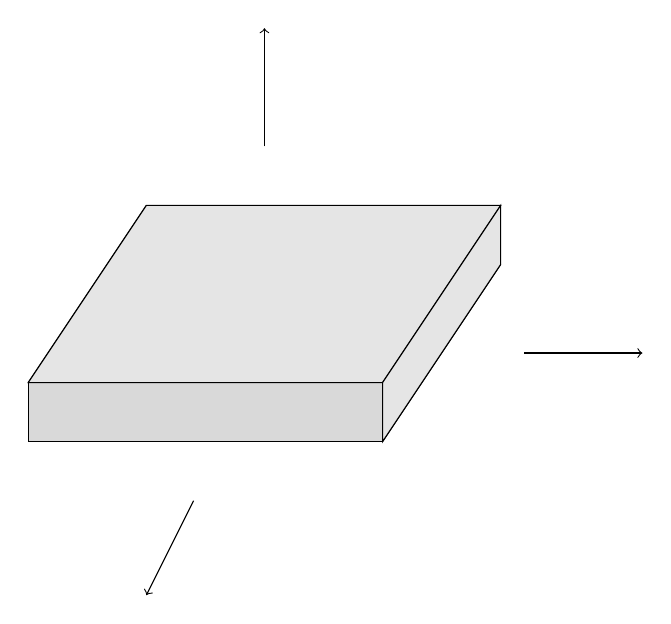
\begin{tikzpicture}[scale=1.5]
		% Face avant
		\draw[fill=gray!30] (0,0) rectangle (3,0.5);
		
		\draw (0,0.5) -- (1,2);
		\draw (3, 0.5) -- (4,2);
		\draw (3,0) -- (4,1.5);
		\draw (4,1.5) -- (4,2);
		\draw (1,2) -- (4,2);
		\draw[fill=gray!20] (0,0.5) -- (3,0.5) -- (4,2) -- (1,2) -- cycle;
		\draw[->] (2, 2.5) -- (2, 3.5);
		\draw[->] (4.2, 0.75) -- (5.2, 0.75);
		\draw[->] (1.4,- 0.5) -- (1,-1.3);
		\draw[fill=gray!20] (3,0) -- (3,0.5) -- (4,2) -- (4,1.5) -- cycle;			
	\end{tikzpicture}
	
	\begin{figure}[H]
		\caption{LSM9DS1 axis  on this card}
	\end{figure}
	
\end{center}

\subsection{Gyroscope}

The STMicroelectronics LSM9DS1 gyroscope is a sophisticated measuring instrument designed to assess rotation rates around the x, y, and z axes. With a typical measurement range of ±245/500/2000 dps, it offers great flexibility to adapt to the specific needs of various applications. \cite{STMicroelectronics_LSM9DS1:2024}

\bigskip 

Operating within a voltage range of 1.71 V to 3.6 V, this gyroscope can seamlessly integrate into different system configurations. Furthermore, its typical operating current ranges from 1 mA to 2 mA, ensuring optimal energy efficiency for battery-powered devices.

\bigskip 

Whether it's for inertial navigation, drone stabilization, or other applications requiring precise motion measurement, the LSM9DS1 gyroscope delivers reliable and accurate performance in a compact and robust form factor, meeting the highest requirements of engineers and designers. 

\bigskip 

\begin{center}
	
	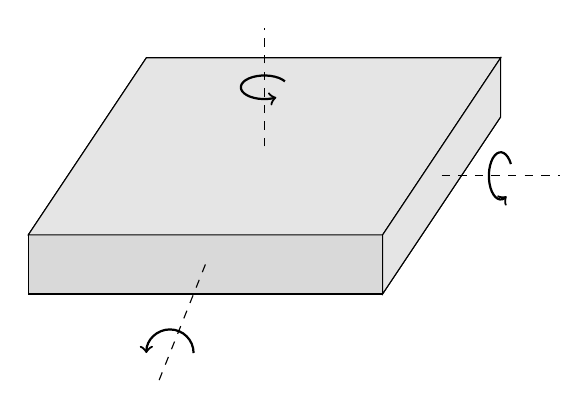
\begin{tikzpicture}[scale=1.5]
		% Face avant
		\draw[fill=gray!30] (0,0) rectangle (3,0.5);
		
		\draw (0,0.5) -- (1,2);
		\draw (3, 0.5) -- (4,2);
		\draw (3,0) -- (4,1.5);
		\draw (4,1.5) -- (4,2);
		\draw (1,2) -- (4,2);
		\draw[fill=gray!20] (0,0.5) -- (3,0.5) -- (4,2) -- (1,2) -- cycle;
		\draw[fill=gray!20] (3,0) -- (3,0.5) -- (4,2) -- (4,1.5) -- cycle;
		\draw[dashed] (2, 1.25) -- (2, 2.25);
		\draw[dashed] (3.5, 1) -- (4.5,1);
		\draw[dashed] (1.5,0.25) -- (1.1,-0.75);
		\draw[thick, ->] (1.4,-0.5) arc[start angle=0,end angle=180,radius=0.2];
		\draw [black, thick, domain=30:300, ->] plot ({2+0.2*cos(\x)}, {1.75+0.1*sin(\x)});
		\draw [black, thick, domain=30:300, ->] plot ({4+0.1*cos(\x)}, {1+0.2*sin(\x)});
	\end{tikzpicture}
	
	\begin{figure}[H]
		\caption{LSM9DS1 axis  on this card}
	\end{figure}
	
\end{center}

\section{Specification}

\subsection{Accelerometer Sensor}

The accelerometer is composed by sensor type MEMS (Micro-Electro-Mechanical Systems) and they used microscopic structures like suspended beams or springs, which deform in response to acceleration. The deformation of these structures is measured using displacement sensors or changes in electrical resistance. MEMS accelerometers are commonly used due to their small size, low power consumption, and comparatively lower cost compared to other types of accelerometers. \cite{pcb_mem_accelerometer:2024}

\bigskip 

The Accelerometer sensor function by \cite{mouser_memssensors:2024} : 

\begin{itemize}
	\item Acceleration Integration for Velocity Estimation: To estimate velocity, the acceleration measured by the accelerometer is integrated over time. Integrating acceleration over time yields velocity.
	
	\item Error Compensation: However, it's crucial to note that acceleration integration is susceptible to cumulative errors. Errors stemming from sensor noise, drift, and inaccuracies can accumulate over time, leading to inaccurate or biased velocity estimates.
	
	\item Utilization of Filters and Sensor Fusion Techniques: To compensate for these errors, advanced techniques such as Kalman filters, Complementary filters, or sensor fusion techniques can be employed. These techniques combine accelerometer data with other sensors such as gyroscopes to enhance velocity estimation accuracy.
	
	\item Calibration and Adjustment: It's also vital to calibrate and adjust the IMU to correct systematic errors and ensure precise measurements. This may involve steps such as compensating for Earth's gravity, correcting gyroscope drift, and reducing sensor noise. 
	
\end{itemize}
\subsection{PIN Conncetion}

They are 4 ways to connect pin, ways depend of what they have after \cite{st_microelectronics_lsm6dso32x:2024}. 

\begin{itemize}
	\item Mode 1: You can utilize either the I\textsuperscript{2}C / MIPI I3CSM slave interface or the SPI (3- and 4-wire) serial interface.
	
	\item Mode 2: This mode supports both the I\textsuperscript{2}C / MIPI I3CSM slave interface or the SPI (3- and 4-wire) serial interface, along with an I\textsuperscript{2}C interface master for external sensor connections.
	
	\item Mode 3: Here, you have the choice of employing either the I\textsuperscript{2}C / MIPI I3CSM slave interface or the SPI (3- and 4-wire) serial interface for the application processor interface. Additionally, an auxiliary SPI (3- and 4-wire) serial interface is designated for external sensor connections, exclusively for the gyroscope.
	
	\item Mode 4: Similar to Mode 3, this mode offers the I\textsuperscript{2}C / MIPI I3CSM slave interface or the SPI (3- and 4-wire) serial interface for the application processor interface. Additionally, it provides an auxiliary SPI (3- and 4-wire) serial interface for external sensor connections, catering to both the accelerometer and gyroscope.	
	
\end{itemize}

\begin{figure}[H]
	\begin{center}
		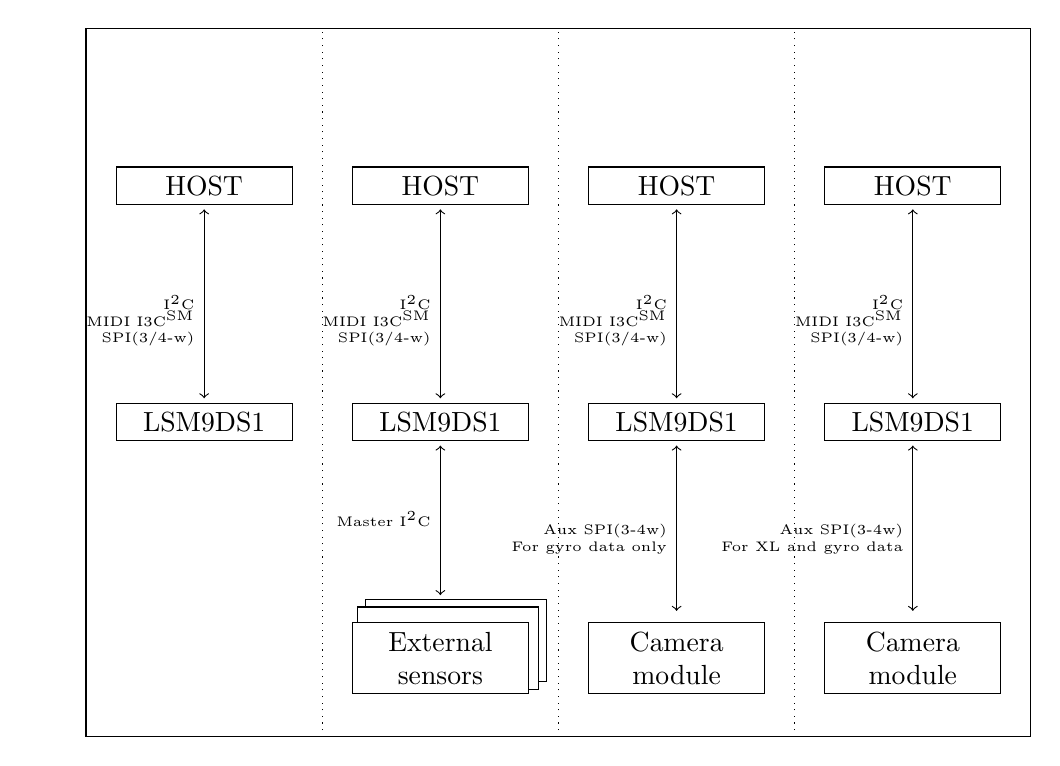
\begin{tikzpicture}
			\draw[fill=white] (0,0) rectangle++(12,9);
			\foreach \x in {3,6,9}{
				\draw[dotted] (\x, 0) -- (\x, 9);}
			\foreach \x in {1.5,4.5,7.5,10.5}{
				\node[draw, fill=white!20, text width=2cm, align=center] at (\x,7) {HOST};
				\node[draw, fill=white!20, text width=2cm, align=center] at (\x,4) {LSM9DS1};}
			\foreach \x in {1.5,4.5,7.5,10.5}{
				\draw[<->](\x,4.3) -- (\x,6.7) node[midway, anchor = mid east, align = right, text width = 2cm, font=\tiny]{I\textsuperscript{2}C\\ MIDI I3C\textsuperscript{SM}\\SPI(3/4-w)};}
			\foreach \x in {7.5,10.5}{
				\node[draw, fill=white!20, text width=2cm, align=center] at (\x,1) {Camera module};
				\draw[<->](\x,1.6) -- (\x,3.7) node[midway, anchor = mid east, align = right, text width = 2cm, font=\tiny]{Aux SPI(3-4w)};}
			\node[anchor=east, align= left, font=\tiny] at (7.5,2.4) {For gyro data only};
			\node[anchor=east,  align= left, font=\tiny] at (10.5,2.4) {For XL and gyro data};
			\draw[fill=white] (3.55,0.7) rectangle++(2.3, 1.05) ;
			\draw[fill=white] (3.45,0.6) rectangle++(2.3, 1.05) ;
			\node[draw, fill=white!20, text width=2cm, align=center] at (4.5,1) {External sensors};
			\draw[<->](4.5,1.8) -- (4.5,3.7) node[midway, anchor = mid east, align = right, text width = 2cm, font=\tiny]{Master I\textsuperscript{2}C};
			
		\end{tikzpicture}
		\caption{Explication of pin mode}  
	\end{center}
\end{figure}





\section{Sensor IMU LSM9DS1}

\subsection{Description}

The LSM9DS1 is a system-in-package featuring a 
3D digital linear acceleration sensor, a 3D digital angular rate sensor, and a 3D digital magnetic sensor.

\subsubsection{Applications}

\begin{itemize}
	\item Indoor navigation.
	\item Smart user interfaces.
	\item Advanced gesture recognition.
	\item Gaming and virtual reality input devices.
	\item Display/map orientation and browsing.
\end{itemize}
\Mynote{citations are missed.}


\subsection{Features}

\begin{itemize}
	\item 3 acceleration channels, 3 angular rate channels, 3 magnetic field channels.
	\item ±2/±4/±8/±16 g linear acceleration full scale.
	\item ±4/±8/±12/±16 gauss magnetic full scale.
	\item ±245/±500/±2000 dps angular rate full scale.
	\item 16-bit data output.
\end{itemize}




\subsection{Pin Connections LSM9DS1}

\begin{figure}[h!]
	\centering	
\includegraphics[width=\linewidth]{Nano33BLESense/imupin}
	\caption{\textbf{Pin connections LSM9DS1}} \cite{STMicroelectronics:2015}
\end{figure}


\subsection{Pin Description LSM9DS1}
\begin{figure}[h!]
	\centering	
\includegraphics[width=14cm]{Nano33BLESense/imupin1}
	\caption{\textbf{Pin description LSM9DS1}} \cite{STMicroelectronics:2015}
\end{figure}

\subsection{Module Specifications}

\subsubsection{Sensor Characteristics}
\begin{figure}[h!]
	\centering	
\includegraphics[width=\linewidth]{Nano33BLESense/sensorchara}
	\caption{\textbf{Sensor Characteristics}} \cite{STMicroelectronics:2015}
\end{figure}


\subsubsection{Temperature Sensor Characteristics}
\begin{figure}[h!]
	\centering	
\includegraphics[width=\linewidth]{Nano33BLESense/tempchara}
	\caption{\textbf{Temperature Sensor Characteristics}} \cite{STMicroelectronics:2015}
\end{figure}

\subsubsection{Absolute Maximum Ratings}

Stresses above those listed as “Absolute maximum ratings” may cause permanent damage 
to the device. This is a stress rating only and functional operation of the device under these 
conditions is not implied. Exposure to maximum rating conditions for extended periods may 
affect device reliability

\begin{figure}[h!]
	\centering	
\includegraphics[width=\linewidth]{Nano33BLESense/absolmax}
	\caption{\textbf{Absolute Maximum Temperature }} \cite{STMicroelectronics:2015}
\end{figure}

\subsection{Block Diagram}

\subsubsection{Accelerometer and Gyroscope Digital Block Diagram}

\begin{figure}[h!]
	\centering	
\includegraphics[width=\linewidth]{Nano33BLESense/acceandgyroblock}
	\caption{\textbf{Accelerometer and gyroscope block diagram}} \cite{STMicroelectronics:2015}
\end{figure}


\subsubsection{Magnetometer Digital Block Diagram}

\begin{figure}[h!]
	\centering	
\includegraphics[width=\linewidth]{Nano33BLESense/magnetometerblock}
	\caption{\textbf{Magnetometer block diagram}} \cite{STMicroelectronics:2015}
\end{figure}

\subsubsection{LSM9DS1 Electrical Connections}

\begin{figure}[h!]
	\centering	
\includegraphics[width=\linewidth]{Nano33BLESense/elecon}
	\caption{\textbf{LSM9DS1 electrical connections}} \cite{STMicroelectronics:2015}
\end{figure}


\subsection{System Requirements}

\fcolorbox{blue}{blue!10}{\begin{minipage}{\textwidth}
		\begin{center}
			\begin{tabular}{llm{90mm}} 
				%\multicolumn{3}{l}{\large \textcolor{blue}{ Tech Specs of Arduino Nano 33 BLE Sense}} \\ \hline
				\\ \textbf{\MapleCommand{\textcolor{blue}{Operating System}}}  & Windows 7 or above, MacOS X or higher \\
				\textbf{\MapleCommand{\textcolor{blue}{CPU}}}  & Intel i3 or above\\
				\textbf{\MapleCommand{\textcolor{blue}{RAM}}}  & Min 2GB\\
				\textbf{\MapleCommand{\textcolor{blue}{Arduino IDE}}}  & V. 1.1819 \\
				\textbf{\MapleCommand{\textcolor{blue}{Boards}}}  & Arduino mBED OS Nano \\
				\textbf{\MapleCommand{\textcolor{blue}{Libraries}}}  & LSM9DS1 \\
				\textbf{\MapleCommand{\textcolor{blue}{Interface}}}  & USB port \\			
			\end{tabular}
		\end{center}
\end{minipage}}

\subsection{Precautions to be taken}


\Mynote{citations are missed}
\begin{itemize}
	
	\item This equipment complies with RF radiation exposure limits set forth for an uncontrolled environment.
	\item This Transmitter must not be co-located or operating in conjunction with any other antenna or transmitter.
	\item The operating temperature of the EUT can't exceed 85$^{0}$C and shouldn't be lower than -40$^{0}$C.
	\item The Frequency band should be in between 863-870Mhz.
	\item Arduino Nano 33 BLE only supports 3.3V I/Os and is NOT 5V tolerant so please make sure you are not directly connecting 5V signals to this board or it will be damaged.
	\item Keep away from water or fire.
	\item Hold it gently, do not harm the components and sensors present on the board.
	
\end{itemize}

%%%%%%%%%%%%%%%%%%%%%%%%%%%%%%%%%%%%%%%%%%%%%%%%%%%%%%%%%%%%%%%%



\section{Libraries}

\subsection{Library Description}

\begin{enumerate}
	\item \FILE{Wire.h} : 	This library is a standard Arduino library that facilitates communication between I\textsuperscript{2}C (Inter-Integrated Circuit) devices. I\textsuperscript{2}C is a synchronous serial communication protocol used to connect microcontrollers to external devices. \FILE{Wire.h} provides functions for initializing the I\textsuperscript{2}C bus, sending and receiving data on the bus, and managing multiple devices on the same bus. With this library, developers can easily connect multiple I\textsuperscript{2}C devices, such as sensors or displays, to an Arduino board. \cite{arduino_wire:2024}
	
	\item \FILE{Kalman.h} : It's a library that implements the Kalman filter algorithm. The Kalman filter is a mathematical technique used to estimate the state of a system from incomplete measurements. It is commonly used in control systems, robotics and navigation applications to improve the accuracy of sensor measurements and reduce errors. \FILE{Kalman.h} provides a simple interface for developers to implement the Kalman filter in their Arduino projects. \cite{arduino_kalman:2024}
	
	\item \FILE{Arduino LSM9DS1.h} :
	The LSM9DS1 library is a software library designed to facilitate interaction with the LSM9DS1 inertial sensor, developed by STMicroelectronics. This sensor combines an accelerometer, a gyroscope and a magnetometer in a single package.The LSM9DS1 library provides an interface for accessing the sensor's functionalities, such as reading acceleration, angular velocity and magnetic field data. It can be used to configure various sensor parameters, such as measurement scales, sampling rates and operating modes. \cite{arduino_lsm9ds1:2024}
	
	
\end{enumerate}

\subsection{Installation}

The bibliographie give coding example for used it, we need to download Arduino Library.  The library \FILE{Arduino LSM9DS1.h} and \FILE{Kalman.h} can be download directly on Arduino. The library \FILE{wire.h} is used if you imput :  include <wire.h>

\begin{center}
	
\includegraphics[width=0.7\linewidth]{Arduino/ArdiunoIDE2/wire}
	\captionof{figure}{Wire include} 
\end{center}



\begin{center}
	
\includegraphics[width=0.7\linewidth]{Arduino/ArdiunoIDE2/LSM6DSboard}
	\captionof{figure}{Board card installation}
	%	\bigskip
\end{center}


\begin{center}	
	
\includegraphics[width=0.7\linewidth]{Arduino/ArdiunoIDE2/LSM9DS1}
	\captionof{figure}{Library choice}
\end{center}


\bigskip



\section{Function}

The LSM9DS1 library on Arduino PortentaH7 is composed of different function. The function is different if you was on I\textsuperscript{2}C protocol or SPI protocol.


\bigskip


\lstdefinestyle{Arduino}{
	language=Arduino,
	basicstyle=\ttfamily\small,
	keywordstyle=\color{blue},
	stringstyle=\color{yellow!30!black},
	commentstyle=\color{green!60!blue},
	morecomment=[l]{//},
	morecomment=[s]{/*}{*/} }

\subsection{Library \FILE{Wire.h}}


This library is used to devellop communication betwin different composent of arduino, it's used for I\textsuperscript{2}C. Wire.h is composed by  \cite{arduino_wire:2024} : 
\begin{itemize}
	
	\item \PYTHON{Wire.begin()}: Initializes the Wire library and prepares the Arduino to act as master or slave on the bus I\textsuperscript{2}C.
	\item \PYTHON{Wire.beginTransmission(address)}: Starts a transmission to a slave device with the specified address.
	\item \PYTHON{Wire.write(data)} : Sends data on the I2C bus during transmission.
	\item \PYTHON{Wire.endTransmission()} : Ends the current transmission and releases the I2C bus.
	\item \PYTHON{Wire.requestFrom(address, quantity)} : Requests data from a slave device with the specified address.
	\item \PYTHON{Wire.available()}: Checks whether data is available to be read after a request.
	\item \PYTHON{Wire.read()}: Reads data received from a slave device.
	
\end{itemize}


\begin{code}
	\lstinputlisting[language=python]{../../Code/Arduino/IMU/WireEx.ino}
	
	\caption{Simple sketch using the sensor LSM9DS1 detection.}\label{TestWire}
	
\end{code}


\subsection{Function \PYTHON{IMU.begin()}}


Calling the function triggers  \PYTHON{IMU.begin()}, the IMU initialization process. This step is important to configures the IMU's basic parameters, establishes communications with other devices, and prepares the unit for proper operation. Accurate initialization is essential to ensure the accuracy and reliability of the data provided by the IMU. \cite{arduino_lsm9ds1:2024}

Incorrect initialization can lead to inaccurate measurements or unpredictable behavior. For example, incorrectly configured measurement parameters or sampling rates can compromise data quality, affecting overall system performance.


\begin{Arduino}
	if (!IMU.begin()) {
		Serial.println("Failed to initialize IMU!");
		while (1);	}
\end{Arduino}


\subsection{Function \PYTHON{IMU.end()}} 

No parameters is required. A return value of 1 indicates that all went well, while a return value of 0 indicates a problem. \cite{arduino_lsm9ds1:2024}

This function is used to stop or deactivate the IMU once it is no longer required. It frees up the resources used by the IMU and ends its operation cleanly. When called, it ensures that all tasks associated with the IMU are properly finalized, avoiding memory leaks or other problems associated with incomplete de-initialization.

This step helps to ensure the stability and reliability of the system as a whole, by avoiding problems associated with incorrect IMU de-initialization.

The data was return at the end. 

\begin{Arduino}
	if (!IMU.begin()) {
		Serial.println("Failed to initialize IMU!");
		while (1); }
	
\end{Arduino}


\subsection{Function \PYTHON{IMU.readAcceleration(x,y,z) }}

IMU accelerometer to retrieve acceleration data, expressed in gravity (g). This function provides information on the movements detected by the IMU's accelerometer. The resulting acceleration data can be used for a variety of applications, such as shock or motion detection, or inertial navigation. By regularly interrogating the accelerometer and analyzing variations in acceleration, it is possible to understand and react to changes in motion with precision, which is essential in many modern embedded systems and electronic devices. \cite{adafruit_lsm9ds1:2024}

The parameters x, y and z are floats giving information on the x, y or z axis 

\begin{Arduino}
	
	float x, y, z;
	
	if (IMU.accelerationAvailable()) {
		IMU.readAcceleration(x, y, z);
		
		Serial.print(x);
		Serial.print('\t');
		Serial.print(y);
		Serial.print('\t');
		Serial.println(z);	}
\end{Arduino}



\subsection{Function \PYTHON{IMU.readGyroscope()}}

Retrieves data from the IMU's gyroscope and returns angular velocity in degrees per second (dps). This function provides information on the rotational movement detected by the IMU's gyroscope. The angular velocity data retrieved can be used in various applications such as robotics, motion tracking or navigation systems. By regularly interrogating the gyroscope and analyzing angular velocity variations, it becomes possible to understand and respond precisely to rotational movements, which is crucial in applications requiring precise orientation control or stabilization. \cite{adafruit_lsm9ds1:2024}

The parameters x, y and z are floats giving information on the x, y or z axis 

\begin{Arduino}
	float x, y, z;
	
	if (IMU.gyroscopeAvailable()) {
		IMU.readGyroscope(x, y, z);
		
		Serial.print(x);
		Serial.print('\t');
		Serial.print(y);
		Serial.print('\t');
		Serial.println(z);	}
\end{Arduino}



\subsection{Function \PYTHON{IMU.accelerationAvailable()}}

This function allows you to check the status of IMU acceleration data, indicating whether or not new data is ready to be retrieved.

In scenarios such as motion tracking, robotics or navigation systems, where the IMU continuously captures acceleration data, the availability of new data determines the system answers. Test the IMU at regular intervals is used for application and they can check for acceleration currently or non, ensuring that the system remains synchronized with object movements in real time. \cite{adafruit_lsm9ds1:2024}

When the function returns a value of 1, this means that new acceleration data is available, enabling the system to extract the data and process it further. A value of 0 indicates that there have been no recent acceleration updates.

\begin{Arduino}
	float x, y, z;
	
	if (IMU.accelerationAvailable()) {
		IMU.readAcceleration(x, y, z);
		
		Serial.print(x);
		Serial.print('\t');
		Serial.print(y);
		Serial.print('\t');
		Serial.println(z); }
	
\end{Arduino}


\subsection{Function \PYTHON{IMU.gyroscopeAvailable()}}

This function ask if new gyro data are available for the IMU and they returns a value 0 if no new gyro data is available, and 1 if new gyro data is ready to be retrieved.

In applications requiring real-time monitoring of rotational motion, such as drone stabilization, virtual reality systems or inertial navigation, the system can determine whether to wait for updated gyroscope readings or proceed to process available data. \cite{Arduino_IMU_Gyroscope:2024}

A value of 1 indicates that new gyro data is available, enabling the system to retrieve and use this information for adapted the orientation tracking or motion control. Conversely, a feedback value of 0 indicates that there have been no recent updates to the gyroscope measurements, prompting the system to wait for new data to become available before proceeding.

\begin{Arduino}
	float x, y, z;
	
	if (IMU.gyroscopeAvailable()) {
		IMU.readGyroscope(x, y, z);
		
		Serial.print(x);
		Serial.print('t');
		Serial.print(y);
		Serial.print(' t');
		Serial.println(z); }
\end{Arduino}


\subsection{Function \PYTHON{IMU.accelerationSampleRate()}}

This function is designed to provide information on the sampling rate of the IMU's accelerometer. The function \PYTHON{IMU.accelerationSampleRate()} returns the accelerometer sampling rate, expressed in Hertz (Hz). This value represents the frequency at which the accelerometer takes measurements and provides acceleration data. It indicates how many times per second the accelerometer registers changes in acceleration along its axes. \cite{STMicroelectronics_LSM9DS1:2024}

In activities such as motion tracking, gesture recognition or vibration analysis, knowledge of the accelerometer's sampling rate ensures that the system can accurately capture and respond to changes in motion dynamics. 

\begin{Arduino}
	Serial.print("Accelerometer sample rate = ");
	Serial.print(IMU.accelerationSampleRate());
	Serial.println(" Hz");
	Serial.println();
	Serial.println("Acceleration in g's");
	Serial.println("X \t Y  \t Z");
\end{Arduino}



\subsection{Function \PYTHON{IMU.gyroscopeSampleRate()}}

To recover and communicate the specific rate at which the gyroscope, integrated into the inertial measurement unit (IMU), collects data samples. This frequency is usually expressed in hertz (Hz), corresponding to the number of samples acquired per second. This is the frequency at which the gyroscope takes measurements, giving an idea of its operational efficiency and performance. \cite{STMicroelectronics_LSM9DS1:2024}

\begin{Arduino}
	Serial.print("Gyroscope sample rate = ");
	Serial.print(IMU.gyroscopeSampleRate());
	Serial.println(" Hz");
	Serial.println();
	Serial.println("Angular speed in degrees/second");
	Serial.println("X tY tZ");
	
\end{Arduino}



\subsection{Library \PYTHON{Arduino\_LSM9DS1}}

Arduino's library \PYTHON{Arduino\_LSM9DS1} for the sensor LSM9DS1 contains three examples that allow the user to use one of the sensors with little effort. \Mynote{missing citation}

\begin{figure}[H]
	\centering
	\includegraphics[width=0.7\textwidth]{IMU/LSM9DS1Bibliothek}
	\caption{Examples in the library \PYTHON{Arduino\_LSM9DS1}}
\end{figure}




\subsection{Installation}

\begin{itemize}
	\item data types
	\item data structure
	\item data quantity
	\item data quality
\end{itemize}

\subsection{Functions}

\section{Example}

In this section, a simple example is described in detail, which demonstrates how the library supports the sensor/actor.


\subsection{Manual}

\subsection{Inside the Example}

\subsection{Code}

\subsection{Files}



\section{Calibration}

cite method

\section{Simple Code}


\section{Simple Application}



\section{Tests}

\subsection{Simple Function Test}

\subsection{Test all Functions}



\section{Further Readings}






%%%%%%%%%%%%%%%
%
% $Autor: Wings $
% $Datum: 2020-01-29 07:55:27Z $
% $Pfad: General/IMUSoftware.tex
% $Version: 1785 $
%
%
%%%%%%%%%%%%%%%






%\section{Bibliotheken}

% Für dieses Projekt wird die Bibliothek \PYTHON{Arduino\_LSM9DS1} des angesprochenen LSM9DS1 benötigt. In dieser Bibliothek sind die Funktionen enthalten, um die Bewegungen zu erfassen und in Winkel umzurechnen. Zusätzlich wird die Bibliothek \PYTHON{SSD1306Ascii}  zur Zeichendarstellung für das OLED-Display benötigt. \Mynote{citations for the libs}
%

\section{Example \FILE{SimpleAccelerometer.ino}}

\subsection{Example's Manual}

\subsection{Inside the Example}

\subsection{Example's Code}






\subsection{Example \FILE{SimpleAccelerometer.ino} - Output}

Das Beispiel \FILE{SimpleAccelerometer.ino}, das von arduino bereit gestellt wird, wurde geladen und der Sensor gibt erfolgreich die Daten der Beschleunigung aus.

\begin{figure}[H]
	\centering
	\includegraphics[width=\textwidth]{IMU/simpleaccelerometer}
	\caption{Output des Testprogramms}
\end{figure}


\subsection{Example's Files}

\FILE{SimpleAccelerometer.ino}


\section{Example - Output on a OLED Display}

\subsection{Programmablaufplan}

\begin{figure}
	\centering
	\includegraphics[width=\textwidth]{IMU/FlowChart}
	\caption{Der Programmablaufplan}
\end{figure}


\subsection{Programmcode und Dokumentation}

\begin{Arduino}
	#include <Arduino_LSM9DS1.h>
	#include <Wire.h>
	#include "SSD1306Ascii.h"
	#include "SSD1306AsciiWire.h"
	
	SSD1306AsciiWire oled;
	
	#define I2C_ADDRESS 0x3C
	#define RST_PIN -1
\end{Arduino}



Mit \PYTHON{\#include} werden die Bibliotheken eingebunden. In diesem Fall werden die Bibliotheken des  Sensors LSM9DS1 und die für das Display erforderliche \FILE{Wire.h} und \FILE{SSD1306Ascii.h} eingebunden. Über \PYTHON{\#define} werden die Adressen festgelegt, damit eine Kommunikation stattfinden kann. 



\begin{Arduino}
	float x, y, z;
	int degreesX = 0;
	int degreesY = 0;
	String yPre, xPre;
\end{Arduino}

Mit \PYTHON{float} (Gleitkommazahl / 4 Bytes) und \PYTHON{Int} (Ganzzahl / 4 Bytes) werden numerische Variablen definiert. In diesem Fall haben wir \PYTHON{degreesX} und \PYTHON{degreesY}, in denen wir unsere jeweiligen X- und Y-Werte für die Ausgabe erhalten. Diese werden zu Beginn auf 0 gesetzt. Die Strings (String=Zeichenkette) \PYTHON{yPre} und \PYTHON{xPre} werden hier implementiert um später die Vorzeichen der X- und Y-Achse zwischen zu speichern.


Nun beginnt das Setup. Hier handelt es sich um eine Funktion, die nur ein einziges Mal aufgerufen wird, sobald der Arduino startet. Da keine Rückgabewerte aus der Methode benötigt werden, wird die Funktionstype \PYTHON{void} verwendet. Die Funktion \PYTHON{Wire.setclock} definiert die Takt Frequenz für die I2C-Kommunikation. 

\begin{Arduino}
	void setup() 
	{
		Wire.begin();
		Wire.setClock(400000L);
		
		#if RST_PIN >= 0
		oled.begin(&Adafruit128x64, I2C_ADDRESS, RST_PIN);
		#else   // RST_PIN >= 0
		oled.begin(&Adafruit128x64, I2C_ADDRESS);
		#endif  // RST_PIN >= 0      
		
		oled.setFont(TimesNewRoman16_bold);
		oled.clear();
		oled.println(" IMU Bereit");
		
		if (!IMU.begin()) 
		{
			oled.clear();
			oled.println("Failed to initialize IMU!");
			while (1);
		}
		
		
		xPre = "   ";
		yPre = "   ";
	}
\end{Arduino}

Die Funktion \PYTHON{oled.setFont} wird verwendet, um die Schriftart und Größe zu ändern. Bei der verwendeten Schriftart handelt es sich um \PYTHON{TimesNewRoman}. Um das Ablesen der Werte zu erleichtern ist die Schriftgröße 16 eingestellt. Der Befehl \PYTHON{oled.println} gibt nach dem Einschalten des Arduinos auf dem Display \PYTHON{''IMU Bereit''} aus. So soll dem Anwender mitgeteilt werden, dass die Messungen gestartet werden können. Falls die IMU nicht einsatzbereit sein sollte, wird über die \PYTHON{if}-Schleife \PYTHON{''Failed to initialize IMU!''} ausgegeben. Mit \PYTHON{xPre} und \PYTHON{yPre} werden aus optischen Gründen drei Leerzeichen definiert. So befinden sich auf der Anzeige die Messwerte geordnet übereinander.



\PYTHON{void loop}  bezeichnet eine Funktion, die jedes mal wenn sie am Ende ist wieder von vorne beginnt. In dieser Schleife werden die Werte, die der Sensor ausgibt, immer wieder aufgerufen und in die entsprechenden Ausgaben eingefügt. Dies sorgt für die Aktualisierung auf dem OLED-Display. 

In der ersten \PYTHON{if}-Abfrage wird abgefragt, ob der X-Wert größer ist als \PYTHON{0.1}. Wenn dies der Fall ist, merkt sich das Programm mit \PYTHON{xPre} das positive Vorzeichen. Die nächsten beiden \PYTHON{if}-Abfragen überprüfen, ob die entsprechenden Werte kleiner gleich 10 Grad sind (siehe Kap. 4.6). Wenn der Y-Wert kleiner gleich 10 Grad ist, gibt das Display die Ausgabe \PYTHON{''  X      0   Grad''} aus. Sobald der Wert größer als 10 Grad ist, beginnt \PYTHON{else} und gibt dem Display die Anweisungen \PYTHON{oled.print(''  X '');} für die Ausgabe des X-Wertes. Unmittelbar dahinter \PYTHON{oled.print(yPre);} für das gemerkte Vorzeichen von Y. Nun wird der vom Sensor gemessene Y-Wert für X eingesetzt \PYTHON{oled.print(degreesY);}. Zum Schluss wird mit \PYTHON{oled.print(''  Grad'');} Grad als Einheit hinter die Zeile gesetzt. Ausgaben wie \PYTHON{oled.print('' '');} beinhalten lediglich eine Leerzeile zur richtigen Ausrichtung der Werte untereinander. Die Funktion \PYTHON{map()} beschäftigt sich mit der Ganzzahlmathematik, dadurch werden selbst Brüche als ganze Zahlen weitergegeben. 

\bigskip

Info: Aufgrund des aufdruckten Koordinatensystems auf dem Gehäuse mussten die X- und Y-Werte getauscht werden, damit es für den Anwender bedienbar ist.


\begin{Arduino}
	void loop() 
	{
		if (IMU.accelerationAvailable()) 
		{
			IMU.readAcceleration(x, y, z);
		}
		if (x > 0.1) 
		{
			x = 100 * x;
			degreesX = map(x, 0, 97, 0, 90);
			
			xPre = "+";
			oled.clear();
			oled.println();
			
			if (degreesY <= 10) 
			{
				oled.println("  X      0   Grad");
			} 
			else 
			{
				oled.print("  X ");
				oled.print(yPre);
				oled.print(" ");
				oled.print(degreesY);
				oled.print("  Grad");
				oled.println();
			}
			if (degreesX <= 10) 
			{
				oled.println("  Y      0   Grad");
			} 
			else 
			{
				oled.print("  Y + ");
				oled.print(degreesX);
				oled.print("  Grad");
				oled.println();
			}
		}      
	\end{Arduino}
	
	Ab der Zeile \PYTHON{if (degreesX <= 10)} erfolgt der gleiche Prozess wie oben beschrieben für den entsprechenden Y-Wert.
	
	Im Folgenden Programmauszug wird die Schleife für die anderen Richtungen wiederholt. Für die X-Werte unter \PYTHON{-0,1} wird mit \PYTHON{xPre = '' -'';} das Vorzeichen gemerkt und die Ausgaben wiederholen sich mit den entsprechenden Vorzeichen und Werten.
	
	\begin{Arduino}
		if (x < -0.1) 
		{
			x = 100 * x;
			degreesX = map(x, 0, -100, 0, 90);
			
			xPre = " -";
			oled.clear();
			oled.println();
			
			if (degreesY <= 10) 
			{
				oled.println("  X      0   Grad");
			} 
			else 
			{
				oled.print("  X ");
				oled.print(yPre);
				oled.print(" ");
				oled.print(degreesY);
				oled.print("  Grad");
				oled.println();
			}
			
			if (degreesX <= 10) 
			{
				oled.println("  Y      0   Grad");
			} 
			else 
			{
				oled.print("  Y  - ");
				oled.print(degreesX);
				oled.print("  Grad");
				oled.println();
			}
		}
		
	\end{Arduino}
	
	
	Hier beginnt die Abfrage für die Y-Werte \PYTHON{if (y > 0.1)}. Sobald das Y positiv ist, wird sich mit \PYTHON{yPre = ''+'';} das Positive Vorzeichen gemerkt und die Schleife läuft wie vorher schon bei den X-Werten beschrieben.
	
	\begin{Arduino}
		if (y > 0.1) 
		{
			y = 100 * y;
			degreesY = map(y, 0, 97, 0, 90);
			
			yPre = "+";
			oled.clear();
			oled.println();
			
			if (degreesY <= 10) 
			{
				oled.println("  X      0   Grad");
			} 
			else 
			{
				oled.print("  X + ");
				oled.print(degreesY);
				oled.print("  Grad");
				oled.println();
			}
			
			if (degreesX <= 10) 
			{
				oled.println("  Y      0   Grad");
			} 
			else 
			{
				oled.print("  Y ");
				oled.print(xPre);
				oled.print(" ");
				oled.print(degreesX);
				oled.print("  Grad");
				oled.println();
			}
		}
		if (y < -0.1) 
		{
			y = 100 * y;
			degreesY = map(y, 0, -100, 0, 90);
			
			yPre = " -";
			oled.clear();
			oled.println();
			
			if (degreesY <= 10) 
			{
				oled.println("  X      0   Grad");
			} 
			else 
			{
				oled.print("  X  - ");
				oled.print(degreesY);
				oled.print("  Grad");
				oled.println();
			}
			
			if (degreesX <= 10) 
			{
				oled.println("  Y      0   Grad");
			} 
			else 
			{
				oled.print("  Y ");
				oled.print(xPre);
				oled.print(" ");
				oled.print(degreesX);
				oled.print("  Grad");
				oled.println();
			}
		}
		delay(50);
	}
	
\end{Arduino}

Hier endet die Schleife. Mit \PYTHON{delay(50)} wird sie alle 50 Millisekunden wiederholt. So wird die Aktualisierung des Displays realisiert. Der Winkelmesser funktioniert also in Echtzeit.\Mynote{Der Begriff Echtzeit ist nicht bekannt. Hier muss gemessen werden!}



\subsection{Anwendung}


Sobald das Programm hochgeladen wurde, gibt es zwei wesentliche Ausgaben auf dem OLED-Display, die der Anwender nun sehen sollte.

\begin{figure}[H]
	\centering
	\includegraphics[width=0.8\textwidth]{OLED/OLEDBereit1}
	\caption{Anzeige des Arduino OLED Displays sobald der Arduino eingeschaltet ist}
\end{figure}

\begin{figure}[H]
	\centering
	\includegraphics[width=0.8\textwidth]{OLED/OLEDBereit2}
	\caption{Ausgabe von Messdaten}
\end{figure}

\PYTHON{X+ 14 Grad, Y+ 12 Grad} ist eine Ausgabe von einer Beispielbewegung des Arduinos und zeigt dem Benutzer eine Mischung aus einem positiven X- und Y-Wert.




\section{Simple Application of code}

\subsection{Initalization example}

In this section, we can see simple code test for sensor LSM9DS1 motion detection as shown in the listing ~\ref{IMU.ino}.


{
	\ArduinoExternalO{../../Code/Arduino/IMU/lsm9ds1.ino}
	
	\captionof{code}{Simple test for sensor LSM9DS1 motion detection}\label{IMU.ino}
}	


\subsection{Application example -- gyroscope application}

In this section, we can see simple code test for gyroscope application as shown in the listing ~\ref{gyrorotattion.ino}.

{
	\ArduinoExternalO{../../Code/Arduino/IMU/gyrorotation.ino}
	
	\captionof{code}{Simple test for gyroscope application}\label{gyrorotattion.ino}
}

\section{Tests}
\subsection{Simple Test Function}
Tests are essential to see the first bases of a code, and to have an answer when you do a part of the code. 

If there's a part of the code where you're stuck in a loop, or something else, testing provides a clear answer to this kind of eventuality. 

When we apply the test, we'll do it with 3 LEDs and test the accelerometer's data acquisition. 

\subsection{Acquisition Test}

In this section, we can see simple test for motion acquisition sensor LSM9DS1 acquisition as shown in the listing ~\ref{TestLSM9DS1.ino}.

{
	\ArduinoExternalO{../../Code/Arduino/IMU/TestLSM9DS1.ino}
	
	\captionof{code}{Simple test for motion acquisition sensor LSM9DS1 acquisition}\label{TestLSM9DS1.ino}
	
}



\section{Calibration}
\subsection{Introduction}

Calibrating an IMU (Inertial Measurement Unit) involves determining the bias, drift, and noise values of the sensors within the IMU. This is achieved by measuring the IMU's output in various positions and orientations, then employing algorithms to calculate the bias, drift, and noise values. This process is crucial to ensure the accuracy of the IMU's measurements. \cite{sugunsegu_imu_calibration:2024}


\subsection{Standard Operating Procedure}

The standard operation procedure for calibrating LSM9DS1 IMU involves the following steps \cite{sugunsegu_imu_calibration:2024} :
\begin{itemize}
	\item Scope and Measurand(s) of Calibrations
	\item Description of the Item to be Calibrated
	\item Measurement Parameters, Quantities, and Ranges to be Determined
	\item Environmental Conditions and Stabilization Periods
	\item Procedure Include:
	\item Handling, transporting, storing and preparation of items
	\item Checks to be made before the work is started
	\item Step by step process
	\item Handling, transporting, storing and preparation of items
	\item Checks to be made before the work is started
	\item Step by step process
\end{itemize}


The signal can be cleaned by different filters using different libraries such as Kalman.


\subsection{Reset part}

Resetting is particularly important for programming purposes or in the event of an external bug. There are 4 main types of programming: 

\begin{itemize}
	\item Soft reset: This method involves using code to trigger a microcontroller reset. For example, in Arduino, this can be done using the reset() function or by executing asm volatile (“jmp 0”). \cite{instructables_reset_arduino:2024}
	\item Hard reset : This method generally involves using an external component, such as a pushbutton or switch, to trigger a hard reset of the microcontroller. This can be achieved by connecting the pushbutton between the RESET pin and ground (GND). \cite{arduino_reset:2024}
	\item Auto Reset: On some Arduino boards, a reset is automatically triggered when a new USB connection is detected. This usually occurs when a new program is downloaded from the Arduino IDE. \cite{stackoverflow_reset_arduino:2025}
	\item Watchdog reset: Some microcontrollers have a built-in “watchdog timer”, which can be used to trigger a reset if the microcontroller remains stuck or unwanted behavior is detected. \cite{youtube_watchdog_reset:2025}
	
\end{itemize}



\subsection{Type of Error}

\begin{enumerate}
	
	\item Bias error : Biases are constant values added to IMU sensor measurements. They can result from various factors, such as inaccuracies in electronic components or variations in the characteristics of the materials used in IMU construction. Biases can be different for each measurement axis (linear acceleration on the x, y and z axes, as well as angular velocity around these axes), and their presence can lead to systematic errors in IMU data. \cite{hexagon_imu:2025}
	
	\item Random walk: Random walk is a noise-type error that manifests itself as random fluctuations in IMU measurements. These fluctuations can be caused by external factors such as vibration or temperature variations. Random deviation can make it difficult to separate the useful signal from the noise in IMU data, particularly when used over long periods of time. \cite{vectornav_random_walk:2025}
	
	\item Gyroscopic drift: Gyroscopic drift occurs when IMU gyroscopes gradually accumulate orientation errors over time. These errors can be caused by  a temperature variations, mechanical vibrations or imperfections in the manufacture of gyroscopic components. Gyroscopic drift can lead to significant errors in IMU orientation estimation, particularly when used over long periods of time without recalibration. \cite{electronics_gyro_drift:2025}
	
	\item Gravity compensation error: When the IMU measures linear acceleration, it must compensate for the gravitational component to obtain accurate measurements. Incorrect gravity compensation can result in orientation errors, particularly when the IMU is used in environments where the direction of gravity varies, such as on board moving vehicles. These errors can lead to inaccuracies in IMU orientation estimates. \cite{advanced_nav_gravity:2025}
	
	\item Sensor synchronization error: If the IMU's sensors are not correctly synchronized, measurement errors may occur. For example, delays or time differences between acceleration and rotation measurements may occur if the sensors are not properly synchronized. These errors can affect the accuracy of IMU orientation and position estimates. \cite{advanced_nav_gravity:2025}
	
	\item Calibration error: Incorrect calibration of IMU sensors can lead to measurement errors. Calibration is the critical process of adjusting sensor parameters to correct systematic errors such as bias and incorrect measurement scales. Inadequate calibration can compromise the accuracy of IMU measurements and lead to incorrect estimates of position, orientation and velocity. \cite{researchgate_calibration:2025}
	
\end{enumerate}

These errors can be mitigated using filtering techniques such as Kalman filters, sensor fusion filters or advanced calibration methods. These methods make it possible to optimally combine information from the IMU's various sensors to obtain more accurate estimates of the position, orientation and velocity of the object to which the IMU is attached. \cite{pmc_kalman_filter:2025}


\subsection{Library \FILE{Kalman.h}}

The \FILE{Kalman.h} library brings together functions essential to the implementation of the Kalman filter, guaranteeing precise filtering and accurate predictions. Each function within this library is designed to handle specific aspects of the filtering process. The library \FILE{Kalman.h}  is an essential tool for signal processing and estimation tasks, enabling reliable and efficient filtering in a variety of applications.  \cite{arduino_kalman:2024}



\subsubsection{Function}

\begin{itemize}
	\item \PYTHON{KalmanFilter.init()}: This function is used to initialize the Kalman filter with necessary parameters, such as the initial state covariance matrix and the process noise covariance matrix, as well as the measurement noise covariance matrix.
	
	\item \PYTHON{KalmanFilter.predict()}: This function is used to predict the future state of the system using the Kalman filter prediction equations. It is typically called at each iteration of the filter, even when new measurements are not available.
	
	\item \PYTHON{KalmanFilter.iupdate()}: This function is used to update the state estimate based on the new available measurement. It utilizes the Kalman filter update equations to combine the predicted estimate with the new measurement.
	
	\item \PYTHON{KalmanFilter.setMeasurementNoise()}: This function allows setting the measurement noise covariance, which represents the uncertainty associated with the measurements provided by sensors.
	
	\item \PYTHON{KalmanFilter.setProcessNoise()}: This function allows setting the process noise covariance, which represents the uncertainty associated with the dynamics of the system.
	
	\item \PYTHON{KalmanFilter.setEstimateError()}: This function allows setting the initial state covariance, which represents the initial uncertainty of the state estimate.
	
	\item \PYTHON{KalmanFilter.getEstimation()}: This function allows retrieving the current estimate of the system state after the update.
	
\end{itemize}

\subsubsection{Kalman filter example}


{
	\ArduinoExternalO{../../Code/Arduino/IMU/KalmanFilter.ino}
	
	\captionof{code}{Simple example with Kalman Filter.}\label{KalmanFilter.ino}
	
}




%%%%%%%%%%%%%%%%%%%%%%%%%%%%%%%%%%%%%%%%%%%%%%%%%%%%%%%%%%%%%%%%%%
